\documentclass{article}
\usepackage[]{amsmath}
\usepackage{pgfplots}
\pgfplotsset{compat=1.18}
\usepackage{amssymb}
%\usepackage[]{pxfonts}
\usepackage[T1]{fontenc}
\usepackage[english]{babel}
\usepackage{tikz}
\usepackage[]{cancel}
\usepackage{listings}
\usepackage{tcolorbox}
\usepackage[ ]{tikz}
\usepackage[ ]{graphicx}
\tikzset{ram grid/.style = {black!100, very thick}}
\tcbuselibrary{listings, skins}

\title{Trabalho Aplicado 1}
\author{Erickson Giesel Müller}
\date{23 de Setembro de 2024}

\begin{document}
\definecolor{codebg}{HTML}{252525}
\definecolor{codetext}{HTML}{ffffff}
\definecolor{codegreen}{HTML}{57db0b}
\definecolor{codeorange}{HTML}{f78e05}
\definecolor{codered}{HTML}{f7052d}
\definecolor{codeshadow}{HTML}{432fa3}

\lstdefinestyle{codestyle}{
	basicstyle =  \color{codetext},
	language = C,
	keywordstyle = \color{codeorange}\bf,
	tabsize = 8
}
\newtcblisting{mylist}{
      enhanced,   %%% needed for shadow
      arc=5mm,
      top=2mm,
      bottom=2mm,
      left=2mm,
      right=10mm,
      boxrule=0pt,
      colback=codebg,
      shadow={1mm}{-1mm}{0mm}{fill=codeshadow,
                      opacity=0.5},             %%% here for shadow  and adjust as you like
      listing only,
      listing options={style=codestyle},
      hbox
}
%\lstset{style=codestyle}
	\maketitle
	\newpage
	
	
	
	\section{Código}
	\begin{mylist}
import sympy

def somaRiemann(funcao, a, b, n):
    x = sympy.Symbol('x')
    f = sympy.sympify(funcao)

    delta_x = (b - a) / n 
    area = 0
    for i in range(n): 
        x_i = a + i * delta_x + delta_x / 2 
        altura = f.subs(x, x_i)
        area += altura * delta_x 
    
    return area


funcao = input("escreva a funcao f(x): ")
a = int(input("Insira o valor de a: ")) 
b = int(input("Insira o valor de b: ")) 
n = int(input("insira o valor de n: ")) 

aprox_area = somaRiemann(funcao, a, b, n)
print("A area aproximada usando a Soma de Riemann 
e: {:.6f} u.a".format(aprox_area))

	\end{mylist}
	Para calcular a aproximação da área abaixo da curva, o código em python usou a biblioteca \textit{sympy}, que fornece diversas ferramentas de álgebra computacional. Para instalar a biblioteca, caso o usuário tenha o python instalado em seu computador, basta rodar no terminal o comando:
	
	\begin{mylist}
pip install sympy
	\end{mylist}
	\newpage
	\section{Soma de Riemann}
	O programa calcula a aproximação da área fazendo a soma das áreas dos \textit{n} retângulos abaixo da curva. Os retângulos tem base $\frac{b-a}{n}$ e altura f(x) no ponto médio. Semelhante à figura abaixo:\\

	\begin{center}
				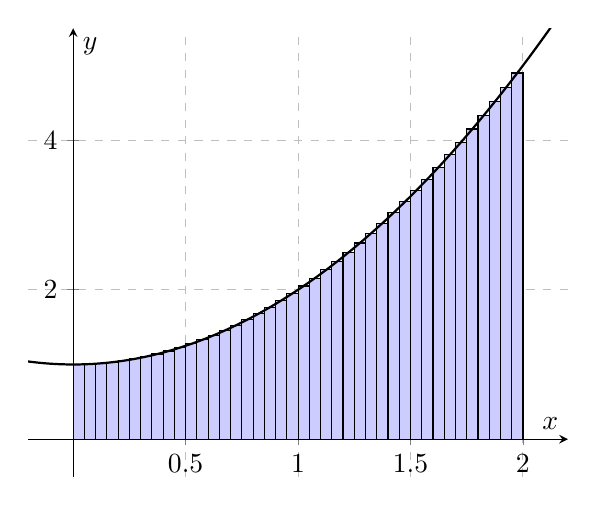
\begin{tikzpicture}
					\begin{axis}[
					    axis lines = middle,
					    xlabel = $x$,
				    	ylabel = $y$,
					    ymin = 0,
					    xmin = 0,
					    xmax = 2,
					    ymax = 5,
					    grid = both,
				    	grid style = dashed,
					    enlargelimits=0.1,
					    samples=500, % Aumentar o número de amostras
					]
						%\addplot[fill=blue!20, domain=0:2] {x^2+1} \closedcycle;
						 % A função correta para a curva azul
						
						% Número de subintervalos (ajuste conforme necessário)
						\pgfmathsetmacro{\n}{10}

						% Largura de cada subintervalo
						\pgfmathsetmacro{\deltax}{0.05}

						% Loop para criar as colunas
						\foreach \i in {0,...,39}{
						    \pgfmathsetmacro{\x}{\i*\deltax + \deltax/2} % Extremo esquerdo do subintervalo
						    \pgfmathsetmacro{\altura}{\x^2+1} % Altura da coluna
						    \addplot[fill=blue!20,thin,domain={\x-\deltax/2:\x+\deltax/2}]{\altura} \closedcycle;
						    %\addplot[fill=blue!20, domain={\x}:\x+\deltax] {\x^2+1} \closedcycle;
						     
						}
						\addplot[color=black, thick] {x^2+1};
					\end{axis}
				\end{tikzpicture}
			\end{center}
	\section{Como operar o programa}
	Para usar o programa no prompt de comando, o usuário deverá escrever:
	\begin{mylist}
python t1-20230001178.py
	\end{mylist}\\
	Em seguida serão solicitadas os dados de entrada:
	$$y;a;b;n$$
	A função é calculada no formato de string, portanto o usuário deverá escrevê-la no seguinte formato:
	\begin{mylist}
a*x**n+b*x**(n-1)+c*x**(n-2)...+z
	\end{mylist}
	Para representar o número $e$, deve-se digitar a letra maíuscula $E$, pois essa é a sintaxe da biblioteca \textit{sympy}.
	\section{Resolução dos problemas:}
		Considerando a função $f(x) = e^{-x}+1$, calcular as aproximações das áreas no intervalo $[-1,1]$ com n subintervalos:
		\subsection{n=4}
			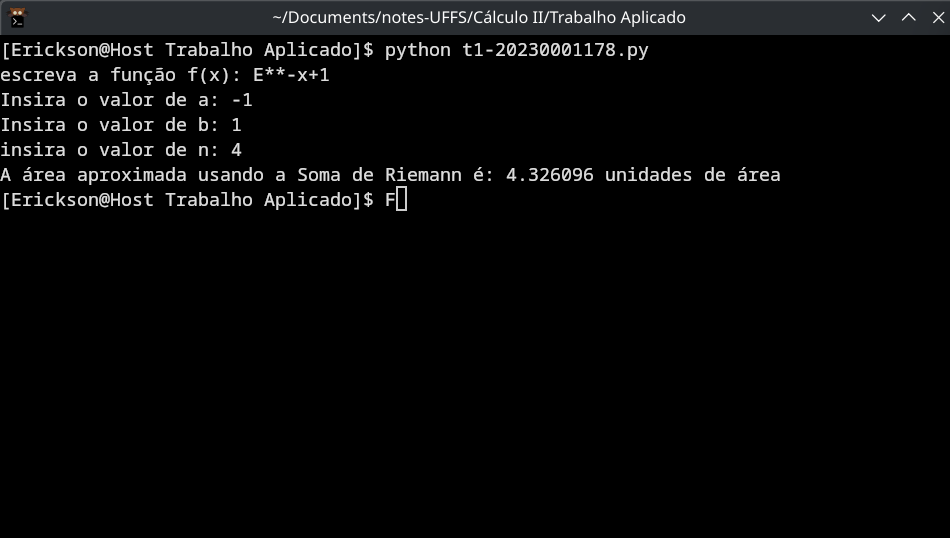
\includegraphics[scale=0.5]{images/n4.png}
		\subsection{n=10}
			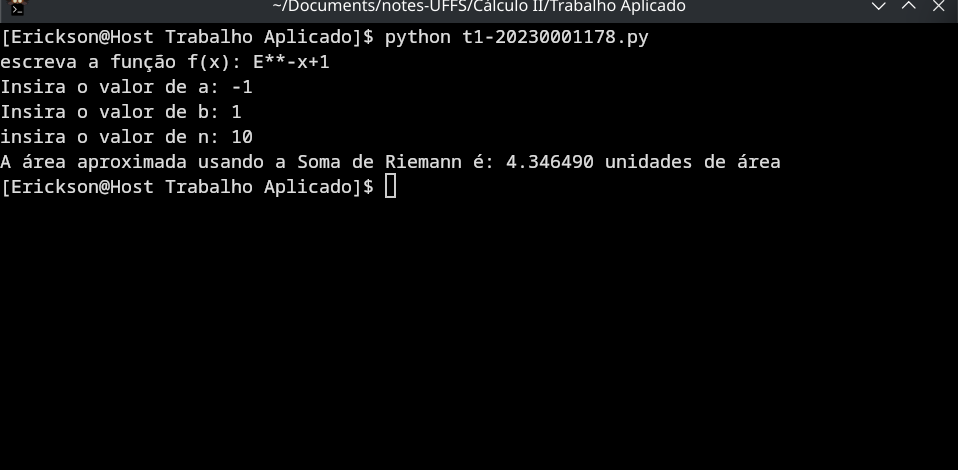
\includegraphics[scale=0.5]{images/n10.png}
		\subsection{n=50}
			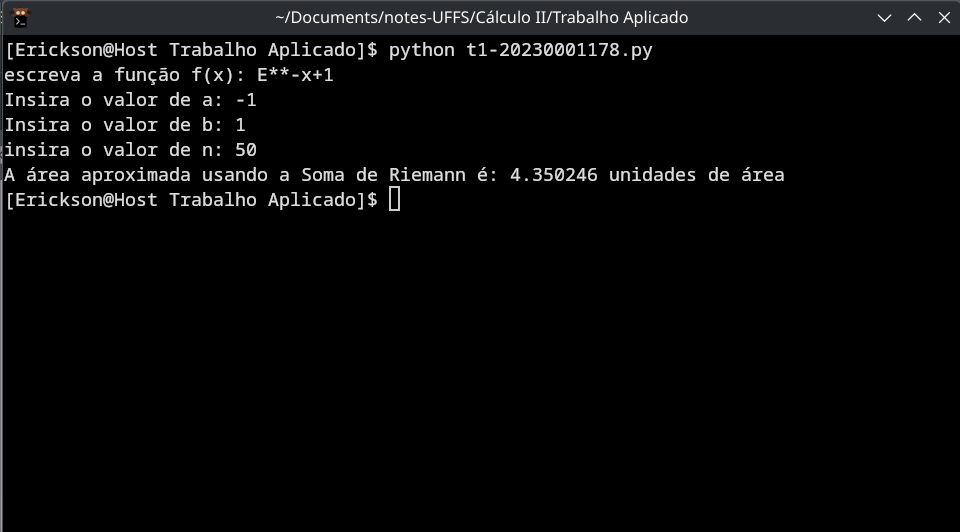
\includegraphics[scale=0.5]{images/n50.png}
		\subsection{n=1000}
			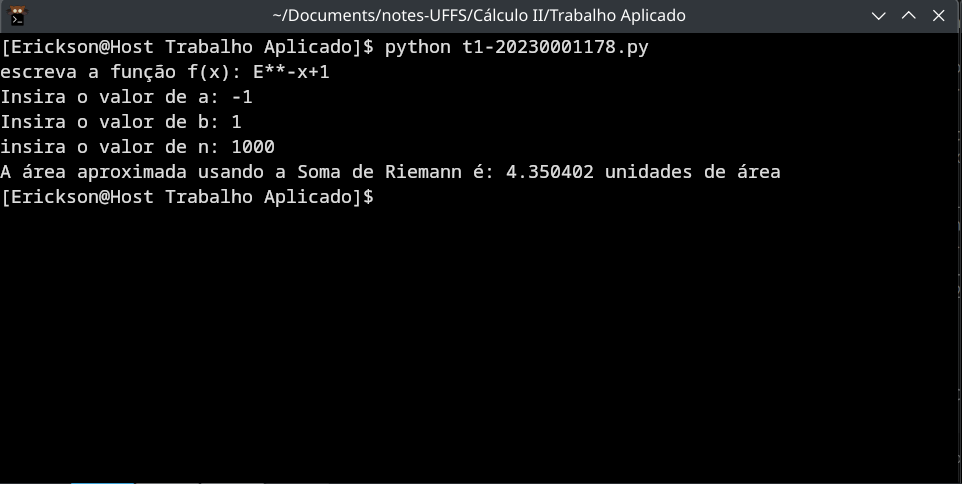
\includegraphics[scale=0.5]{images/n1000.png}
	\section{Considerações Finais}
		Analisando os resultados, percebemos que quanto maior o número de subintervalos, mais preciso será o resultado da aproximação em relação à integral. Isso acontece porque na àrea dos retângulos que está sendo calculada, há uma área de imprecisão das partes dos retângulos que estão à esquerda e à direita do ponto médio da base. Essa imprecisão é reduzida conforme a largura da base dos retângulos diminui, e estes pontos ficam cada vez mais próximos da curva. \\
		Conforme a fórmula da Soma de Riemann, percebe-se que o resultado fornecido pelo programa fica cada vez mais próximo do valor exato da integral conforme o número de subintervalos aumentam.Também, quanto maior for número de subintervalos, mais sutil será a diferença se comparado com o resultado de um valor $n$ próximo, por esse motivo o resultado é entregue com 6 casas decimais.
		$$\int_{a}^{b}f(x).dx = \lim_{x\to +\infty}\sum_{i=1}^{h}f(C_i).\Delta x$$
		Utilizando os valores do exemplo acima:\\
		$$y = e^{-x}+1$$
		$$Area = \int_{-1}^{1} [e^{-x}+1].dx=[x-e^{-x}]_{-1}^{+1}$$
		$$[1-e^{-1}]-[-1-e^1]=2+e-e^{-1}$$
		$$Area \approx 4.35040238729 u.a$$
		Portanto, para essa função, sob essas condições, o programa conseguiu atingir um resultado preciso com 1000 subintervalos.
		
\end{document}